\section{System model \& problem statement}

\begin{figure}
    \centering
    \begin{subfigure}{\columnwidth}
        \centering
        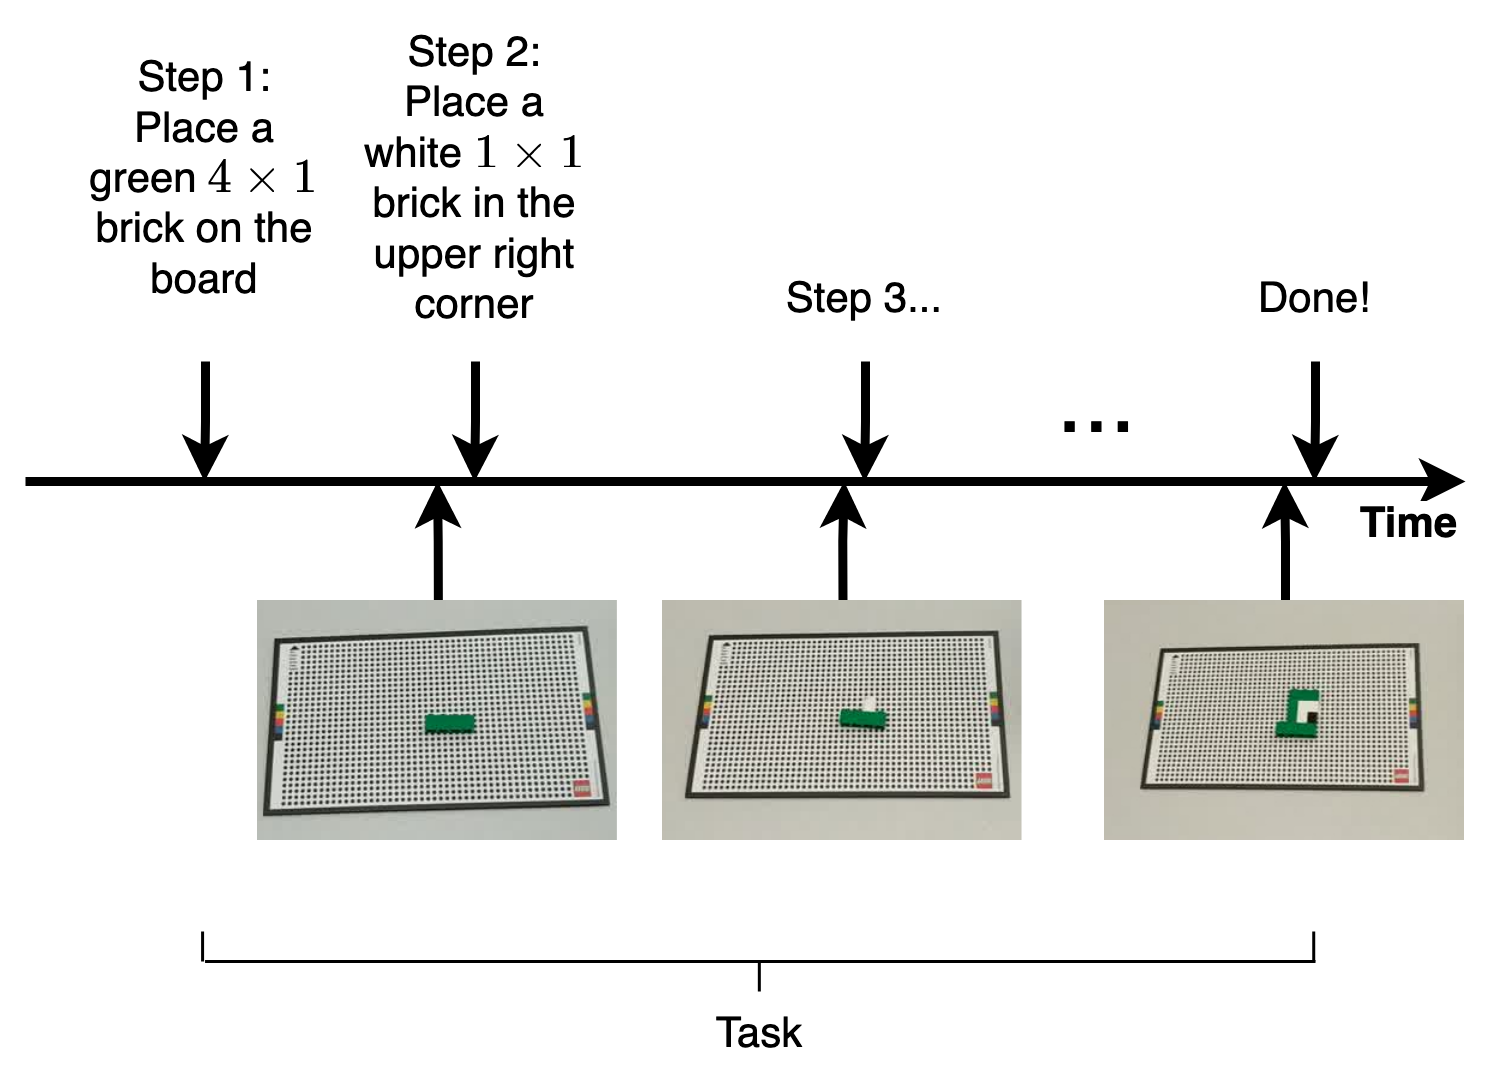
\includegraphics[width=.9\textwidth]{figs/task}
        \caption{%
            Overview of a task in a \gls{WCA}, composed of a series of steps.
            Each steps starts with an instruction being provided to the user and ends with the instruction for the next step.
            The \gls{WCA} continuously samples the task state, automatically triggering transitions between steps as correct (or incorrect) states are recognized.
        }\label{fig:task}
    \end{subfigure}\\
    \begin{subfigure}{\columnwidth}
        \centering
        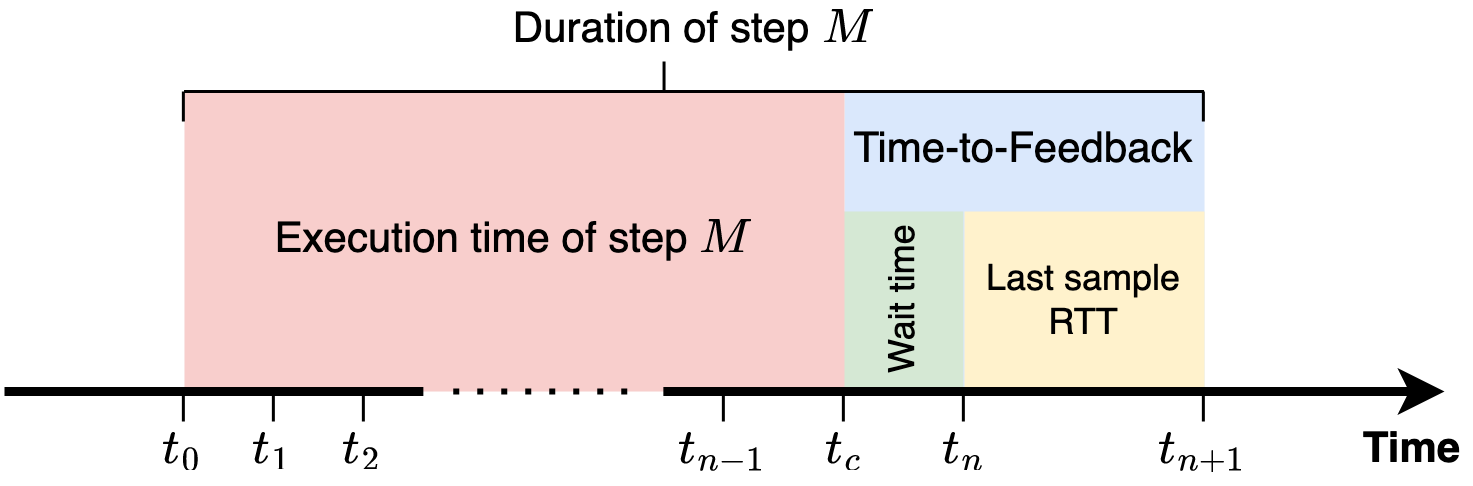
\includegraphics[width=.9\textwidth]{figs/step_time}
        \caption{%
            Breakdown of a step into its timing components.
            The instruction for step \( M \) and \( M + 1 \) are provided to the user at \( t_0 \) and \( t_{n+1} \), respectively.
            \( t_k | k \in \{1, \ldots, n \} \) correspond to the \gls{WCA} sampling instants for step \( M \), and \( t_c \) marks the instant at which the user finishes performing the instruction.
        }\label{fig:step}
    \end{subfigure}
    \caption{Key concepts in \gls{WCA}}
\end{figure}

\glsreset{WCA}

\todo[inline]{Add table of terms?}

We consider in this work a \gls{WCA} application deployed on a terminal-server system.
\gls{WCA} applications represent a category of novel, context-sensitive and highly-interactive \gls{AR} applications.
We focus on a particular category --- ``step-based'' \gls{WCA} --- that have as their goal the guiding of a user through a sequential task.
Examples of such applications are the LEGO and IKEA assistants~\cite{chen2015early,chen2018application}, in which users are guided step-by-step through the process of assembling a LEGO model and an IKEA lamp, respectively.

Step-based \glspl{WCA} operate analogously to how \gls{GPS} navigation assistants guide users, by seamlessly and continuously monitoring the progress of the user and autonomously providing relevant instructions and feedback.
The application follows the progress of the task in ``realtime'' by repeatedly sampling the state of the physical system, most commonly through video frames.
Whenever the assistant detects that the user has correctly or incorrectly performed an instruction, it provides a new instruction to either advance the task or correct the detected mistake.
The application otherwise remains silent and out-of-the-way of the user;
that is, samples which do not generate a new instruction (e.g.~because they captured an intermediate or unfinished state, or simply noise) are silently discarded, and only an acknowledgement is provided to the terminal device.
This acknowledgement is simply for flow control of samples, and the user is not aware of it.
Herein lies one of the key characteristics of these applications: the user only consciously interacts with the application whenever they finish an instruction, and thus these are the \emph{only} points in time at which they can notice changes in system responsiveness.

We formally define a \emph{step} as a specific action to be performed by the user, described by a single instruction. 
A \emph{task} consists of a series of steps to be executed in sequence (refer to \cref{fig:task}).
A step begins when the corresponding instruction is provided to the user, and ends when the instruction for the next step is provided; we call the time interval between these two events the \emph{step duration}.

\glspl{WCA} employ sampling, most commonly of video feeds, to continuously monitor the state of the real world.
Let \( \{ t_0, t_1, \ldots, t_{n + 1} \} \) represent a series of discrete and sequential sampling instants when the \gls{WCA} captures the state of the physical system, as depicted in \cref{fig:step}.
\( t_0 \) corresponds to the instant when the instruction for step \( M \) is provided and the first sample is taken. 
\( t_n \) indicates the instant when the final sample capturing the state of \( M \) is taken. 
\( t_{n + 1} \) represents then instant when the result for sample \( t_n \) is returned and the instruction for step \( M + 1 \) is provided.
The total number of samples captured is denoted by the random variable \ensuremath{\mathcal{S}}.

In this context, we define \( t_c \) as the point in time at which the user finishes performing the instruction for step \( M \).
We denote the interval \( t_c - t_0 \) as the step \emph{execution time}, represented by the random variable \ensuremath{\mathcal{T}}) and \( t_n - t_c \) as the step \emph{wait time}, represented by the random variable \ensuremath{\mathcal{W}}.
Finally, \( t_{n + 1} - t_n \) corresponds to the \gls{RTT} of the last sample of step \ensuremath{M}.
The sum of the wait time and the last sample \gls{RTT} (i.e.\ the interval \( t_{n + 1} - t_c \)) we term \emph{\gls{TTF}}, which represents a metric used throughout this paper to describe the responsiveness of a \gls{WCA}.
We also note here that whereas \ensuremath{\mathcal{T}} we consider a system property, \ensuremath{\mathbb{S}} and \ensuremath{\mathcal{W}} are derived from \ensuremath{\mathcal{T}} and the selection of sampling instants.

An ideal sampling policy for \gls{WCA} samples the system immediately after \ensuremath{t_c}, resulting in a wait time of zero and a \gls{TTF} equal to the \gls{RTT} of this sample.
It is evident, however, that such a policy is not possible to implement in reality due to the randomness of \ensuremath{\mathcal{T}}.
Instead, we must design a policy that achieves a balance between the expected number of samples \ensuremath{\mathbb{E}\mathcal{S}]} and the expected wait time \ensuremath{\mathbb{E}\mathcal{W}]}.
From~\cite{moothedath2022energy2} we know that, in general, any objective metric $\mathcal{E}$ in these applications which relates to sampling and the responsiveness of the system will present itself as a linear combination between $\mathbb{E}[\mathcal{S}]$ and $\mathbb{E}[\mathcal{W}]$ plus terms independent of the number of samples or wait time:
\begin{alignat}{1}
    \Rightarrow\mathcal{E}&=\alpha\mathbb{E}[\mathcal{S}]+\beta\mathbb{E}[\mathcal{W}]+C\;\label{eq:epsilon_terminal}
\end{alignat}

To obtain expressions for \ensuremath{\alpha} and \ensuremath{\beta} that result in \ensuremath{\mathcal{E}} representing the energy consumption due to sampling in a step, we directly take the modeling from~\cite{moothedath2022energy2} with a necessary modification in the assumption of one-way communication in all but the final sample.
Feedback is given even to to the discarded samples in our model, albeit hidden from the user.
We therefore expand the definition of the communication delay \ensuremath{\tau_\text{c}} from~\cite{moothedath2022energy2} to include the total delay in either direction, retaining \ensuremath{\tau_\text{p}} as the backend processing time of each sample, and \( P_\text{c} \) and \( P_0 \) as the energy consumed per unit of time at the terminal during communication and when idle, respectively.
These terms allow us to express the energy consumption due to sampling of a step as
\begin{alignat}{2}
    \mathrm{E}=&\;\mathcal{S}\tau_cP_c+(\mathcal{T}+\mathcal{W}+\tau_\mathrm{p}+\tau_\mathrm{c}-\mathcal{S}\tau_c)P_0\nonumber\\
    % &=s\tau_c(P_c-P_0^{(t)})+wP_0^{(t)}+(\tau+\tau_c+\tau_p) P_0^{(t)}+\tau_cP_c\\
    =&\;\tau_{\text{c}}(P_{\text{c}} -P_0)\mathcal{S}+\mathcal{W}P_0+(\mathcal{T}+\tau_{\text{p}} +\tau_{\text{c}}) P_0\label{eq:energy_expr}
\end{alignat}
Taking the expected value of \cref{eq:energy_expr} allows us to drop the last term, as it has a constant expectation for a given distribution of \ensuremath{\mathcal{T}},
\begin{gather}
    \mathbb{E}[\mathrm{E}] = \tau_{\text{c}}(P_{\text{c}} - P_0)\mathbb{E}[\mathcal{S}]+P_0\mathbb{E}[\mathcal{W}]+ C\nonumber\\
    \intertext{resulting in the following expressions for \ensuremath{\alpha} and \ensuremath{\beta}}
    \alpha=\tau_{\text{c}}(P_{\text{c}} -P_0),\text{ and }\beta=P_0\;\blacksquare\nonumber
\end{gather}


In this work, as in~\cite{moothedath2022energy2}, we aim to find an aperiodic sampling policy that minimizes \cref{eq:epsilon_terminal} when \ensuremath{\mathcal{E}} represents the energy consumption due to sampling of a step in a \gls{WCA}.
However, our focus lies not in the finding of a theoretical optimum --- as this has already been achieved --- but in how such a solution materializes as a practical implementation.
The optimal sampling policy presented in~\cite{moothedath2022energy2} presents characteristics that make it a challenge to implement in real systems.





% It should be noted 
% it must follow that (see also~\cite{olguinmunoz:impact2021})\footnote{\( U(a, b) \) represents the continuous uniform distribution in the open interval \( (a, b) \).}
% % \todo[inline]{I think it's an assumption rather than a must. Specifically, it is not uniform if the general execution time distribution is Rayleigh/ExpGaussian -vishnu}
% \begin{align}\label{eq:tc}
%     t_c &\thicksim U(t_{n - 1}, t_n)
% \end{align}

% Current implementations, such as those in~\cite{Chen2015LEGO,Chen2018application}, employ \emph{greedy} sampling.
% In this scheme, a new sample is immediately taken as soon as an acknowledgement is received for the previous sample.
% This means that the interval between these sampling instants is not necessarily constant, as it is subject to fluctuations due to resource contention on both the network and compute side.
% It also has as a consequence that acknowledgements must be provided even for those samples which do not cause the generation of a new instruction --- these acknowledgements are simply used for flow control and do not generate user-noticeable feedback.


